\section{Discussion}

\begin{frame}
  \frametitle{Discussion}


\begin{columns}
\begin{column}{0.5\textwidth}

Estimated performance:
$$1\:\mathbf{Byte}*10\:\mathbf{MHz}= 80\:\mathbf{Mbps}$$
% \item<3>Usability
% \item<4>Using C\#
% \end{itemize}
\end{column}

\begin{column}{0.5\textwidth}

Improving the performance:
\begin{figure}
\centering


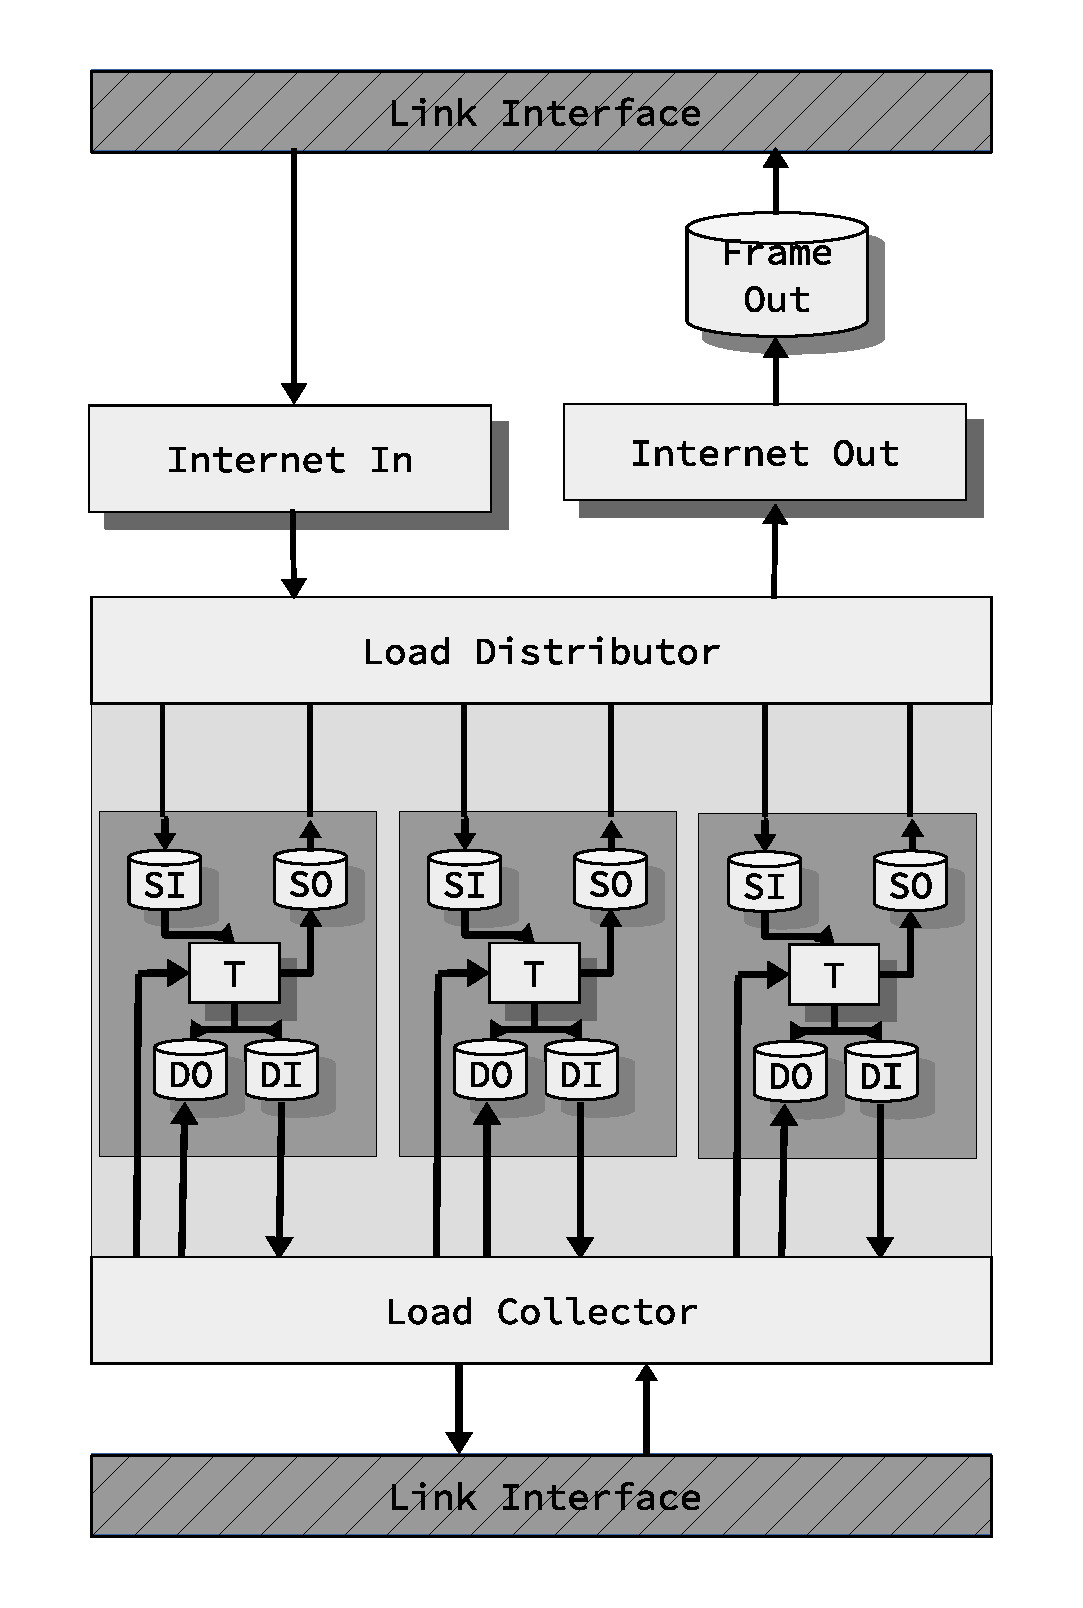
\includegraphics[scale=0.25]{../thesis/discussion/design_stacked.eps}
\end{figure}
\end{column}
\end{columns}

\end{frame}


\begin{frame}
\begin{columns}
\begin{column}{0.5\textwidth}
Usability

\end{column}

\begin{column}{0.5\textwidth}
SOMETHING
\end{column}
\end{columns}
\end{frame}

\begin{frame}
\begin{columns}
\begin{column}{0.5\textwidth}
Using C\#
\end{column}

\begin{column}{0.5\textwidth}
State modelling\\
Simulation\\
Concurrency
\end{column}
\end{columns}
\end{frame}

\section{Conclusion}
\begin{frame}
  \frametitle{Conclusion}

\begin{itemize}
\item Lot of trial and error to find the optimal design in the beginning
\item In 10 mio. simulated clock cycles, 17283 packets were handled,  1280 of
which were correctly received by the Application layer, and then sent out
again
\item Even with a few flaws, SME is a great framework for hardware modelling
\end{itemize}

\end{frame}
